
\documentclass[letterpaper,11pt]{article}
\usepackage[utf8]{inputenc}
\usepackage[spanish]{babel}
\usepackage{mathtools}
\usepackage{graphicx}
\usepackage{hyperref}

\begin{document}

\title{Estructura de datos\\\LargeÁrboles $B$\\\small Actividad 8}
\author{Dagoberto Quevedo}
\maketitle

\begin{abstract}
En esta actividad se describen las propiedades y funcionalidades de los árboles $B$, complementando con el uso de la librería \texttt{BTree} en Python para realizar una implementación computacional que apoye en la formulación de un diseño experimental que evalúe el rendimiento de la estructura.
\end{abstract}

\section{Árboles $B$}

Los árboles $B$ son una generalización de los árboles binarios que resultan eficiente en un modelo de acceso de memoria. Para cualquier entero $B \ge 2$, un árbol $B$ es un árbol en el que todas las hojas tienen la misma profundidad y cada nodo no raíz, $u$, tiene al menos $B$ hijos y como máximo $2B$ hijos. Los hijos de $u$ se almacenan la lista, $c^u$. El número de hijos permitidos por nodo es entre 2 y $ 2B $ hijos. En los árboles $B$ aplica para la altura $\ell$ del árbol que  $B \ge 2$,

\begin{equation}
	h\le \log_{B} \frac{n+1}{2},
\end{equation}

Si la altura de un árbol $B$ es $h$, entonces se deduce que el número, $\ell$, de hojas en el árbol $B$ es,

\begin{equation}
	2B^{h-1}\le \ell \le 2(2B)^{h-1}.
\end{equation}

Es decir, la altura de un árbol $B$ es proporcional al logaritmo base $B$ del número de hojas. Cada nodo $u$, en $ B$  almacena una lista de claves $c^u_i,\dots,c^u_{2B-1}$. Si $u$ es un nodo interno con $k$ hijos, entonces el número de claves almacenadas en $u$ es exactamente $k-1$ y se almacenan en $c^u_1,\dots,c^u_{k-2}$. Las claves en un árbol $B$ se representan de manera similar que en un árbol de búsqueda binario. Dado un nodo, $u$ que almacena las claves $k-1$,

\begin{equation}
	c^u_1 < c^u_2,\dots,c^u_{k-2}
\end{equation}

Búsqueda de una clave en un árbol $B$ es distinto a una operación de búsqueda de un árbol binario, sólo que en esta clase de árboles se tendrá que elegir entre distintas alternativas en cada nodo intermedio. La siguiente figura muestra un ejemplo de árbol $B$,

\begin{figure}[h!]
  \centering
  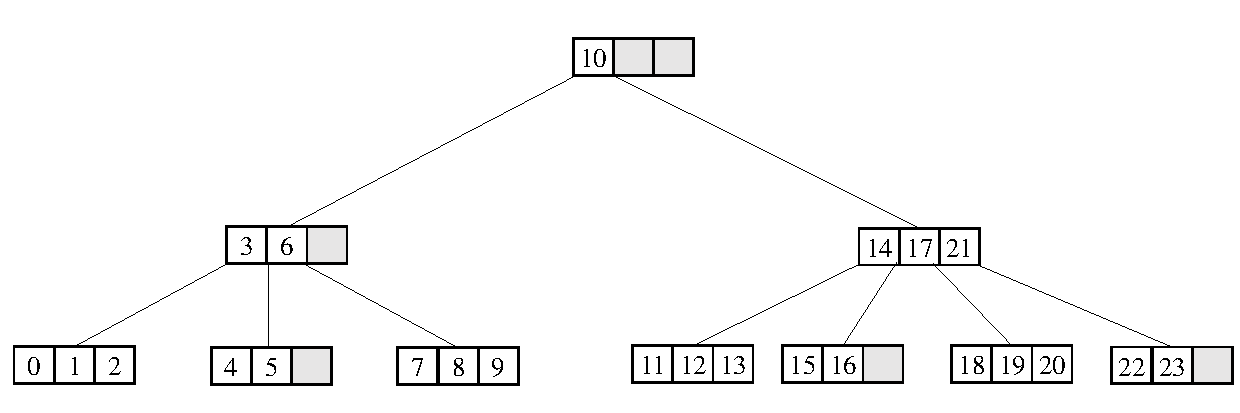
\includegraphics[width=\textwidth]{img/btree.pdf}
  \caption{Ejemplo de un árbol $B$, con $B=2$.}
  \label{fig:ie}
\end{figure}

Se deduce que los datos almacenados en un nodo de un árbol $B$ tienen un tamaño $O(B)$. Por ejemplo, si las claves son números enteros de 4 bytes y los índices del nodo también son 4 bytes, entonces establecer $ B=256 $ significa que cada nodo almacena $\displaystyle (4+4)\times 2B= 8\times512=4096$ bytes.

\subsection{Implementación computacional}

Se hace uno de la librería \texttt{BTree} para la implementación computacional; el diseño experimental consiste en la la creación aleatoria de árboles $B$, con valores dados en un rango de número enteros y medir su eficiencia en la búsqueda de casos extremos, así como el tamaño de las estructuras en la memoria.


\begin{thebibliography}{0}
 \bibitem{Btrees2020} \textit{Open Data Structures}, 14.2 B-Trees, \url{opendatastructures.org/ods-python/14_2_B_Trees.html}
  \bibitem{Knuth1998} Donald Knuth, \textit{Sorting and searching}, The Art of Computer Programming, Addison-Wesley Professional, 1998.
  \bibitem{Schaeffer2020} Elisa Schaeffer, \textit{Modelos computacionales}, Complejidad computacional de problemas y el análisis y diseño de algoritmos, notas de curso, 2020.
\end{thebibliography}


\end{document}
